\documentclass[12pt, a4paper]{report}
\usepackage[utf8]{inputenc}
\usepackage{graphicx}
\usepackage{nameref}
\graphicspath{ {Pictures/} }
\usepackage{hyperref}
\hypersetup{
    colorlinks=true,
    linkcolor=blue,
    filecolor=magenta,      
    urlcolor=red,
}
\usepackage{geometry}
\usepackage{float}
\usepackage{algorithm}
\usepackage{algpseudocode}
\usepackage{amsmath, bm}
\usepackage[export]{adjustbox}
\usepackage{subcaption}
\usepackage{mathabx}
 

\title{%  
Homework Assignment 3 
   \\
  \large  Dynamics Of Non Linear Robotic Systems}
\author{Ilia Sevostianov %\thanks{thanks to God}
    }
\date{\today}

\begin{document}
	\maketitle


\section*{Task 1:}
Derive FK equations for the robot depicted in figure \ref{fig:mesh1}. Use $\theta_1$, $\theta_2$, $d_3$ as
joint space variables, $p_x$, $p_y$, $p_z$ as operational space variables. Parameters
$d_1$, $a_2$ are known (assign them some positive values for succeeding tasks).

\begin{figure}[H]
	\centering
		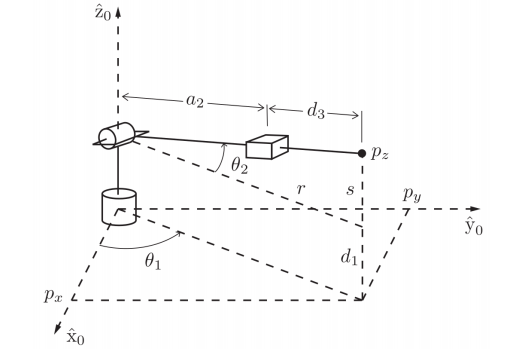
\includegraphics[width=0.6\textwidth]{Image1} % File
	\caption{RRP robot.} % Name
	\label{fig:mesh1}
\end{figure}

\section*{Task 2} \label{sec:Task 2}
 Derive IK equations.


\section*{Task 3:}
Compute the manipulator Jacobian for representation of linear and angular velocity of point \textbf{p}.
\begin{itemize}
	\item Use classical approach (partial derivatives).
\item Use geometric approach (cross products).
\end{itemize}


\section*{Task 4:}
Analyze the Jacobian for singularities. Characterize each singular configuration if any.


\section*{Task 5:}
Compute the velocity of the tool frame when joint variables are changing with time as follows:

{\centering
$\theta_1(t) = sin(t)$, $\theta_2(t) = cos(2t)$, $d_3(t) = sin(3t)$.
}

Add some fancy graphs showing evolution of all variables



\section*{Task 6:}
Let tool coordinates changing with time as follows:

{\centering
$p_x(t) = 2a_2sin(t)$, $p_y(t) = 2a_2cos(2t)$, $p_z(t) = d_1sin(3t)$
}

Determine a feasible joint trajectory for this tool trajectory.

\begin{itemize}
	\item Use IK solution.
	\item Use inverse differential kinematics approach. Consider only linear
velocity part of Jacobian.
\end{itemize}


\end{document}